\chapter{PCB} \chapterlabel{Informe/8-PCB} \label{cap:PCB}

\section{PCB}

\subsection{Fuentes de Alimentación}

\subsubsection{Fuente de alimentación externa de 24V}

\noindent La fuente externa se encarga de alimentar todo el circuito. Debe ser capaz de suministrar 24V y hasta 30A. Para ello se puede utilizar una fuente de laboratorio o baterías.

\subsubsection{Fuente de alimentación interna de 12V}

\noindent La fuente de 12V se encarga de alimentar al regulador de 5V y al driver del puente H. Debido a los bajos consumos de potencia y bajo costo, se utiliza una fuente lineal. Por lo tanto, se decide utilizar el integrado L78M12CDT-TR.

\subsubsection{Fuente de alimentación interna de 5V}

La fuente de 5V se encarga de alimentar los operacionales, el sensor de efecto hall, el inversor y el regulador de tensión de 2.5V. Debido a los bajos consumos de potencia y bajo costo, se utiliza una fuente lineal. Por lo tanto, se decide utilizar el integrado L78M05CDT.

\subsection{Esquemáticos}

\subsubsection{Main}
\begin{figure}[H]
	\centering
	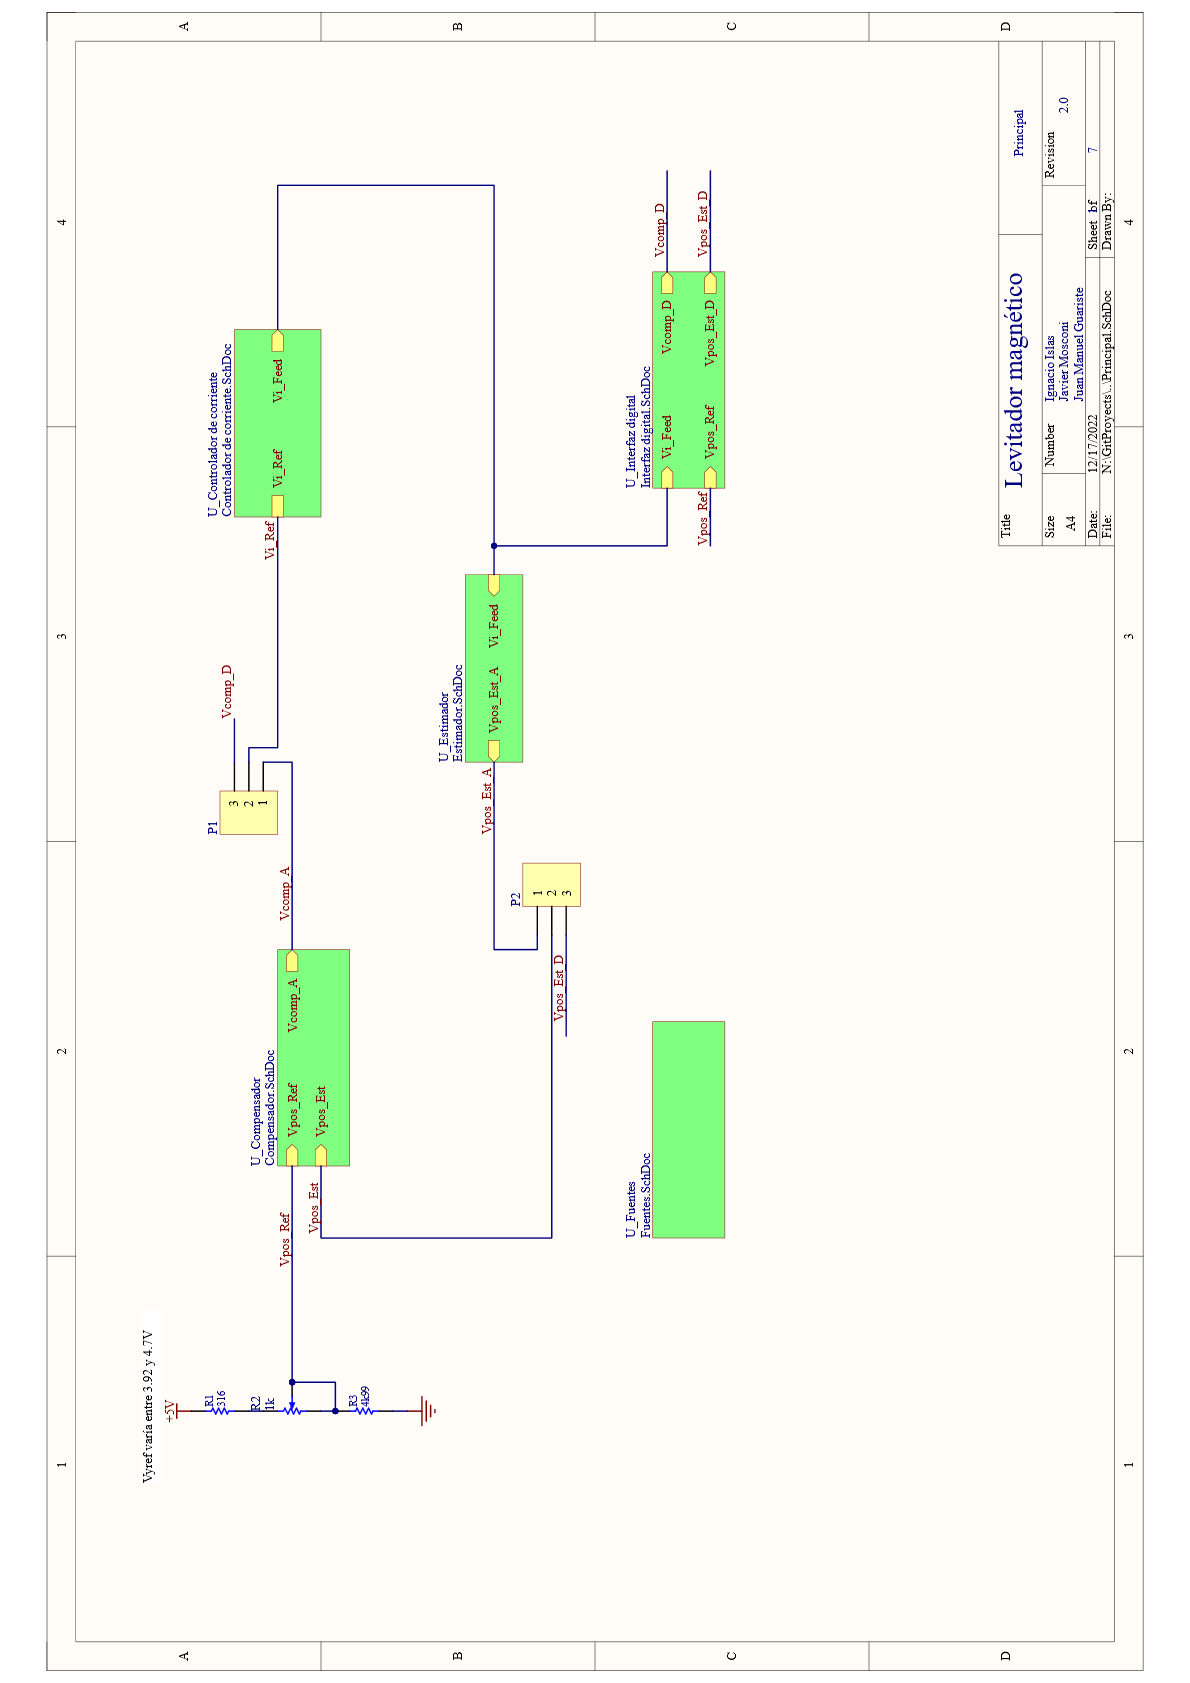
\includegraphics[scale=0.3]{main.png}
	%\caption{Diagrama en bloques de la implementación digital.}
	\label{fig:main}
\end{figure}

\subsubsection{Controlador de corriente}
\begin{figure}[H]
	\centering
	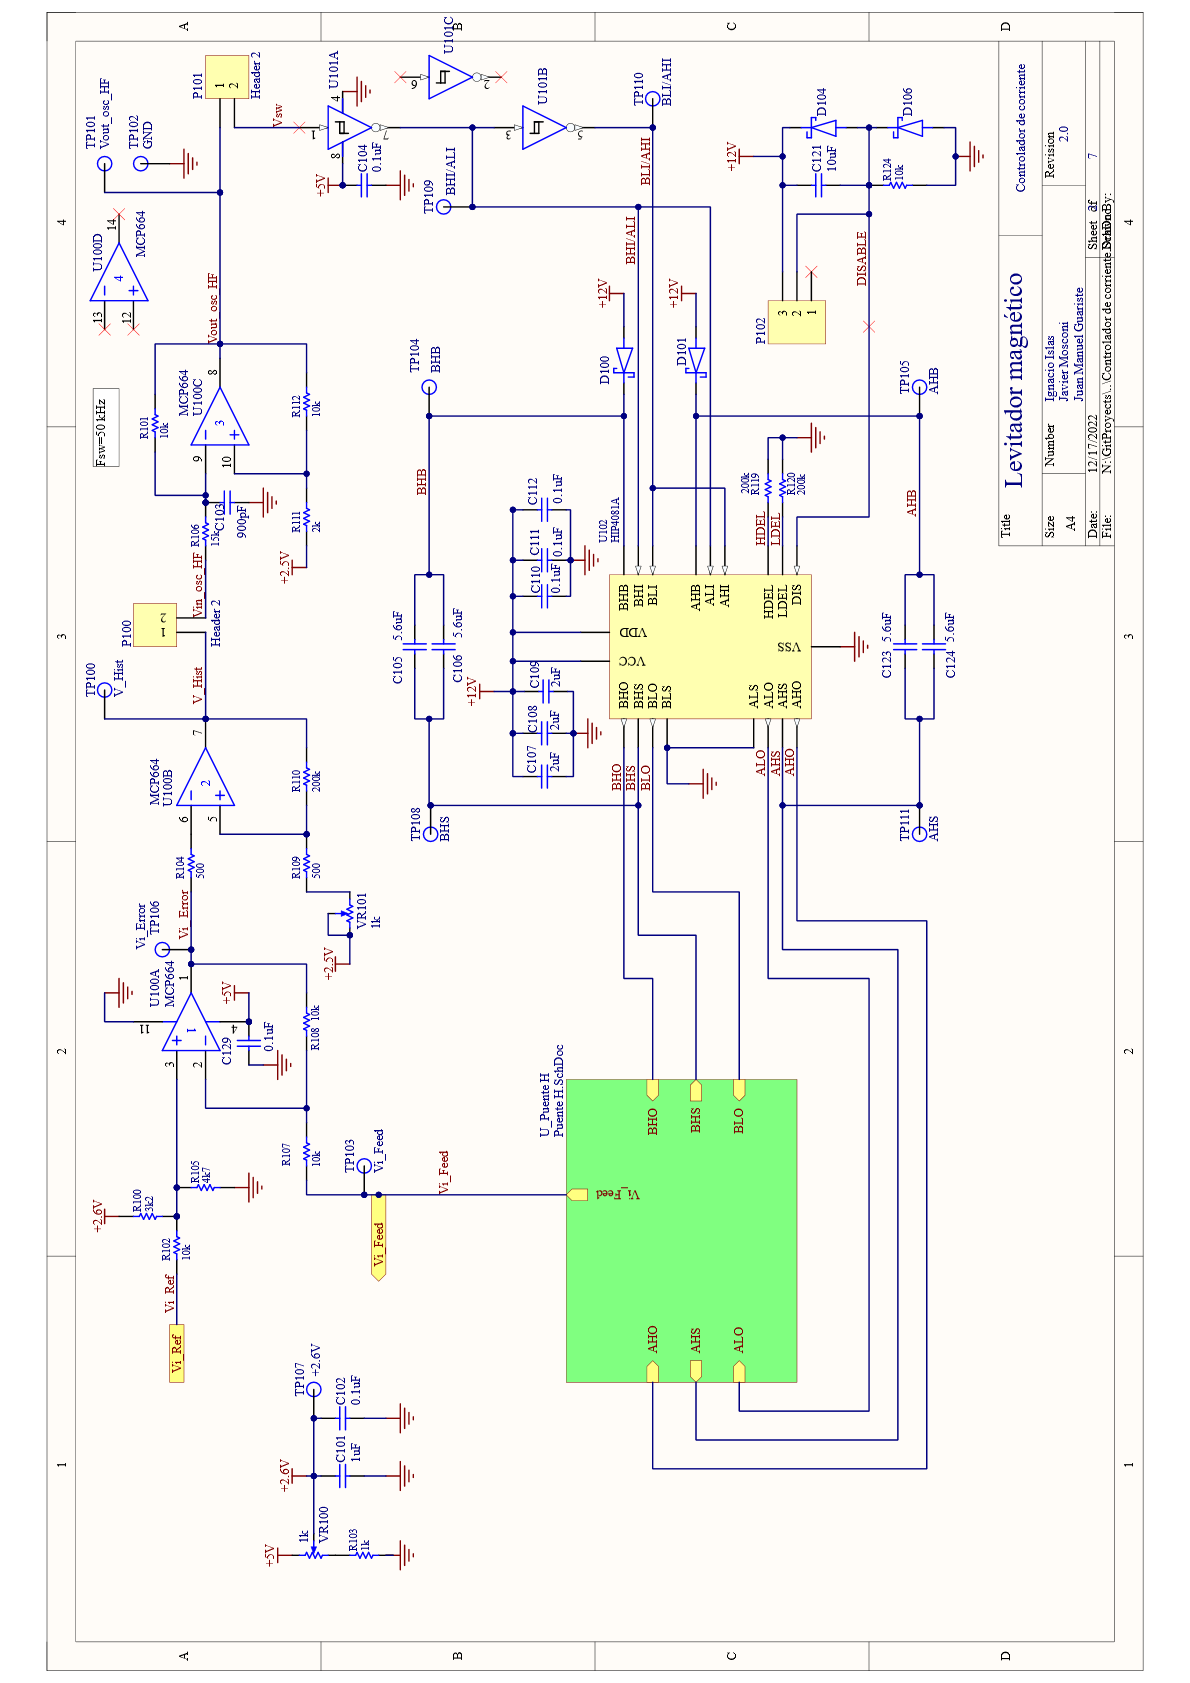
\includegraphics[scale=0.32]{contCorrEsq.png}
	%\caption{Diagrama en bloques de la implementación digital.}
	\label{fig:contCorrEsq}
\end{figure}

\subsubsection{Puente H}
\begin{figure}[H]
	\centering
	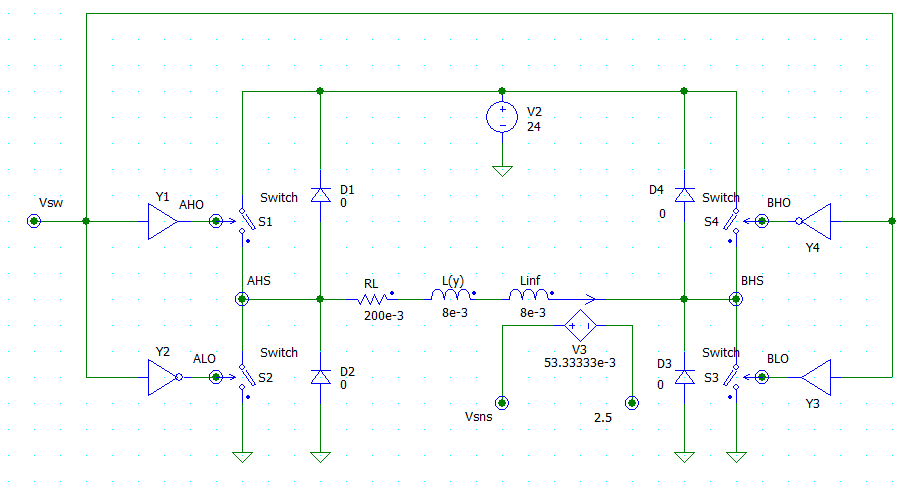
\includegraphics[scale=0.32]{PuenteH.png}
	%\caption{Diagrama en bloques de la implementación digital.}
	\label{fig:PuenteH}
\end{figure}

\subsubsection{Compensador analógico}
\begin{figure}[H]
	\centering
	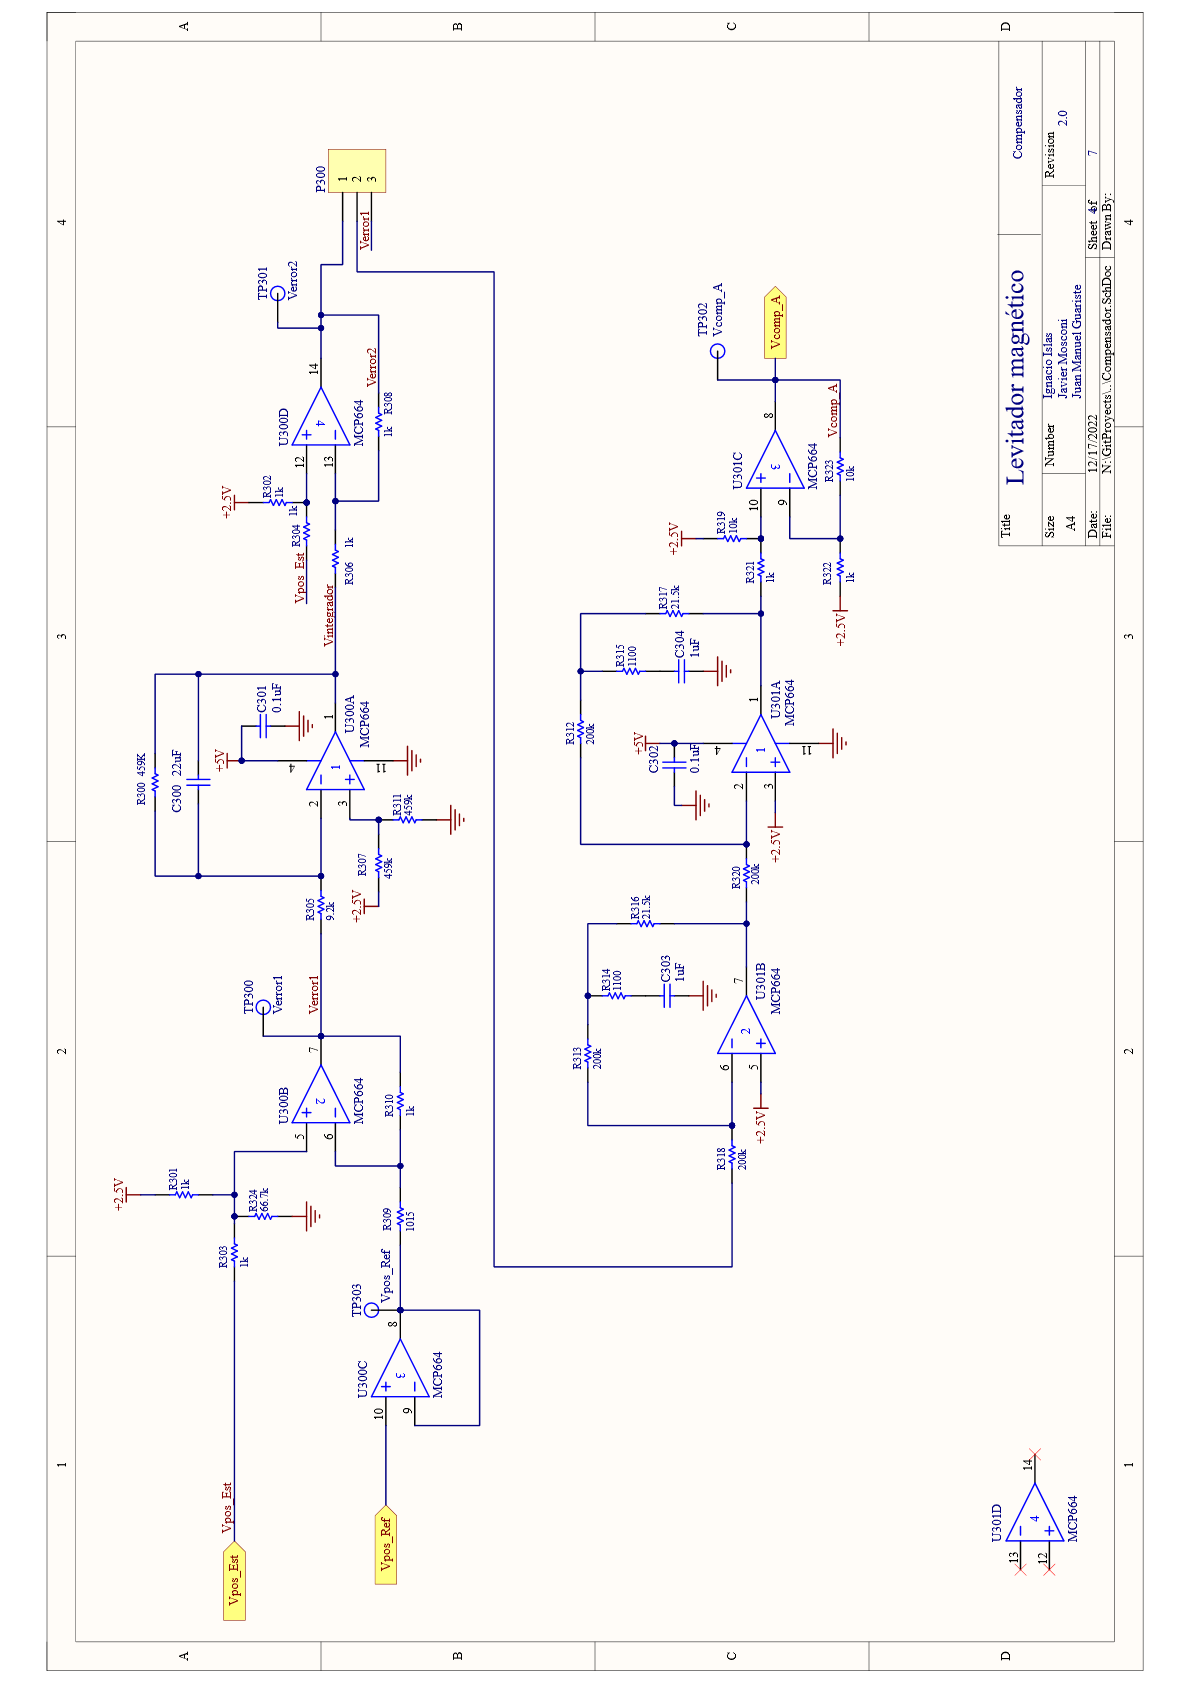
\includegraphics[scale=0.32]{CompAnalog.png}
	%\caption{Diagrama en bloques de la implementación digital.}
	\label{fig:CompAnalog}
\end{figure}

\subsubsection{Estimador analógico}
\begin{figure}[H]
	\centering
	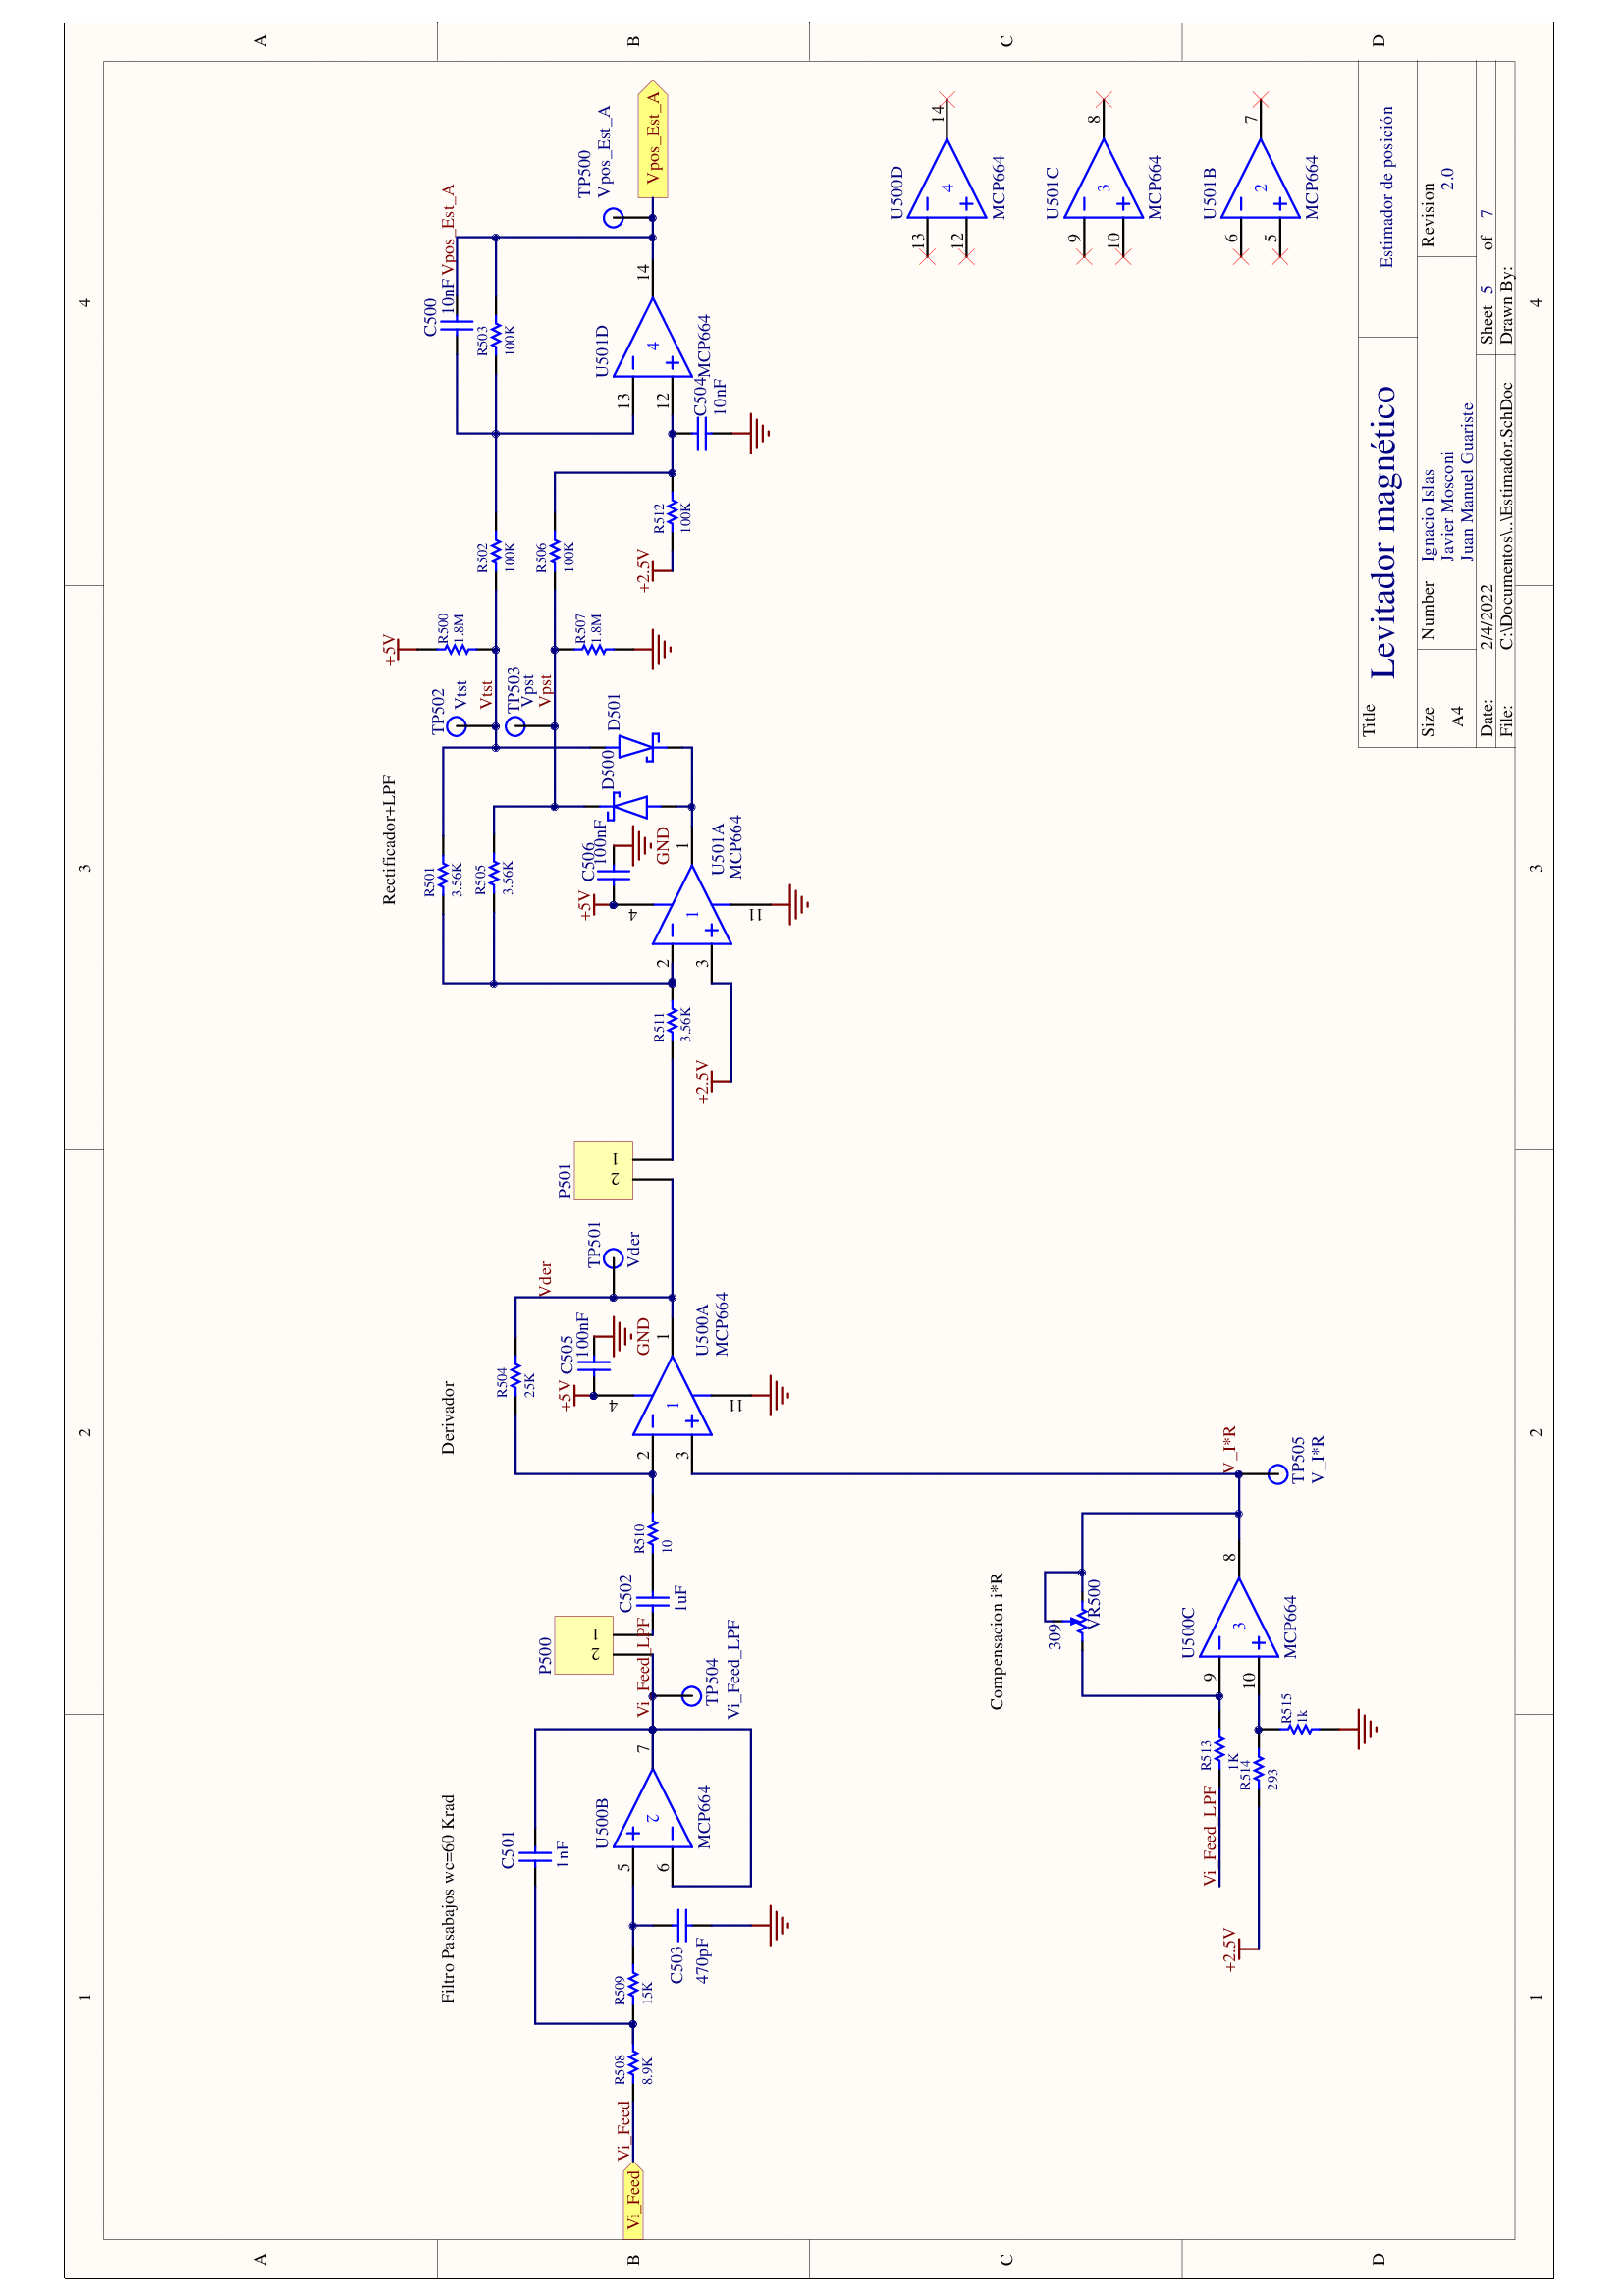
\includegraphics[scale=0.32]{EstimAnalog.png}
	%\caption{Diagrama en bloques de la implementación digital.}
	\label{fig:EstimAnalog}
\end{figure}

\subsubsection{Interfaz con microcontrolador}
\begin{figure}[H]
	\centering
	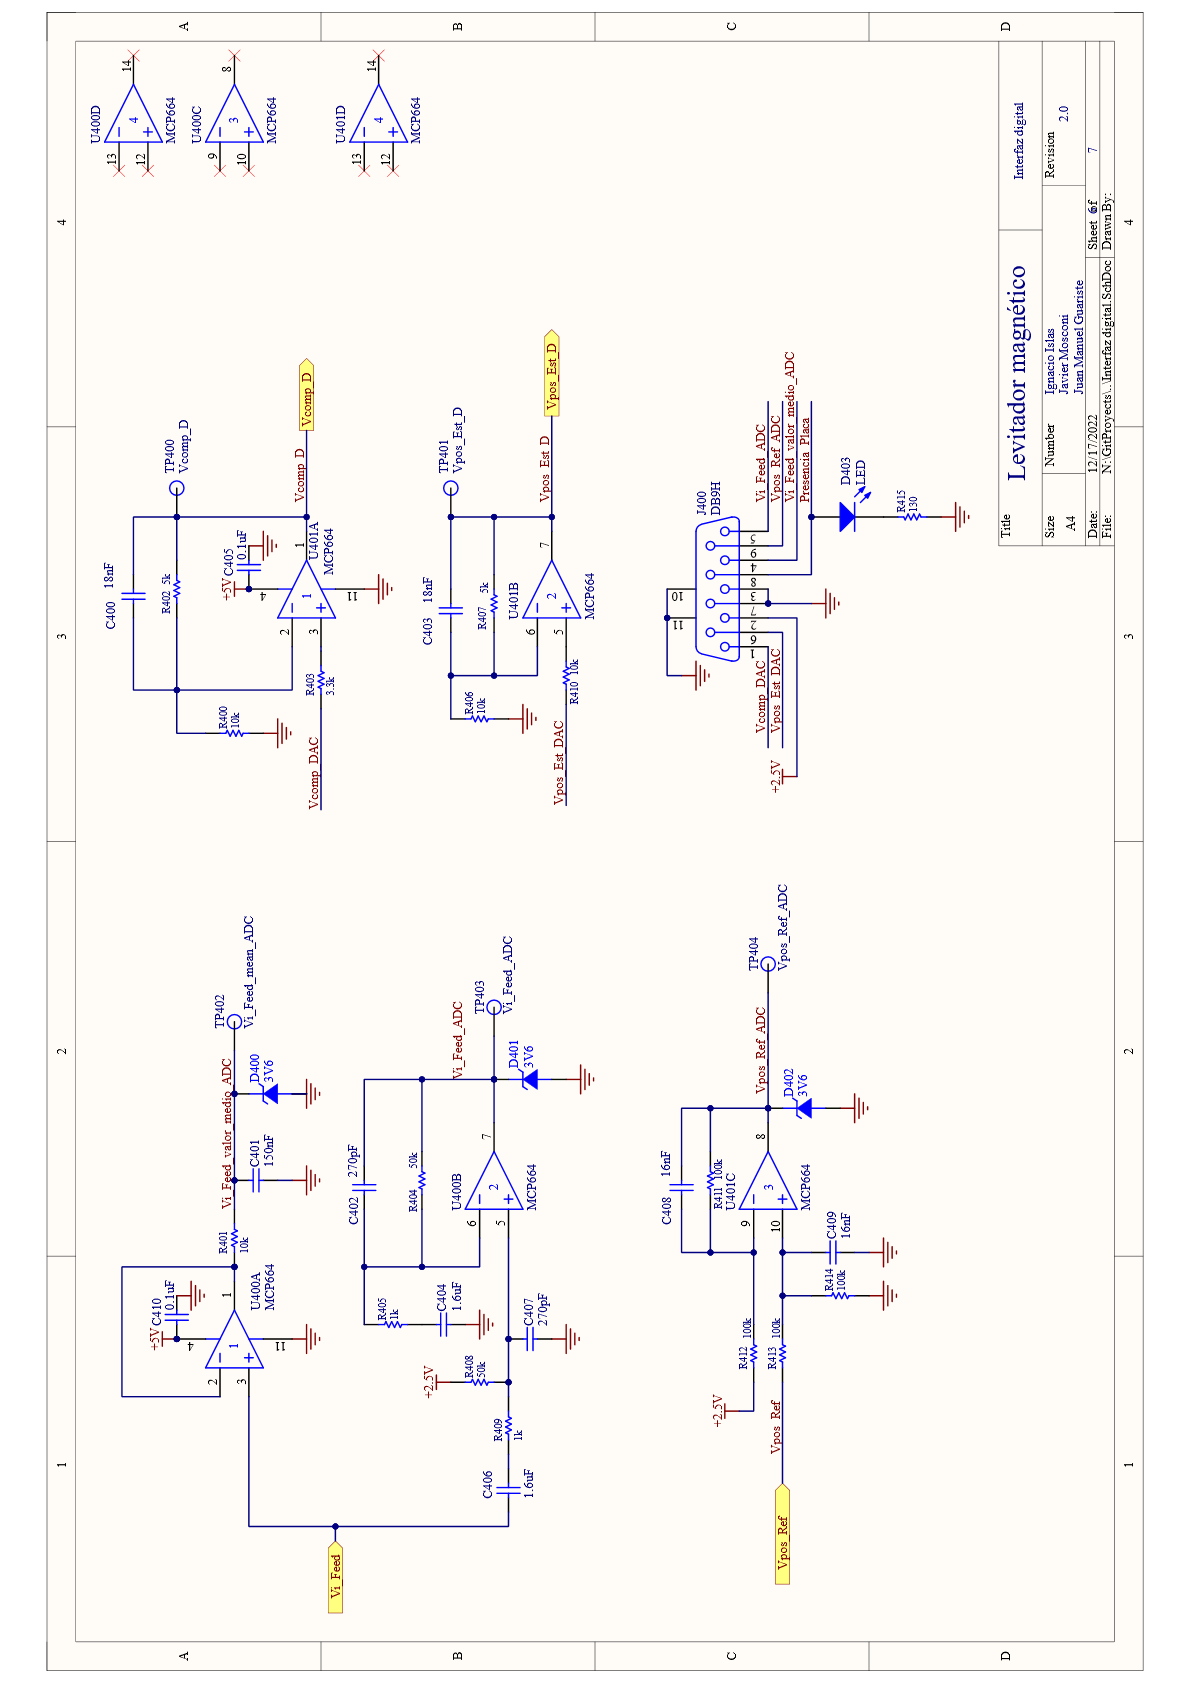
\includegraphics[scale=0.32]{InterfazMic.png}
	%\caption{Diagrama en bloques de la implementación digital.}
	\label{fig:InterfazMic}
\end{figure}

\subsubsection{Fuentes de alimentación}
\begin{figure}[H]
	\centering
	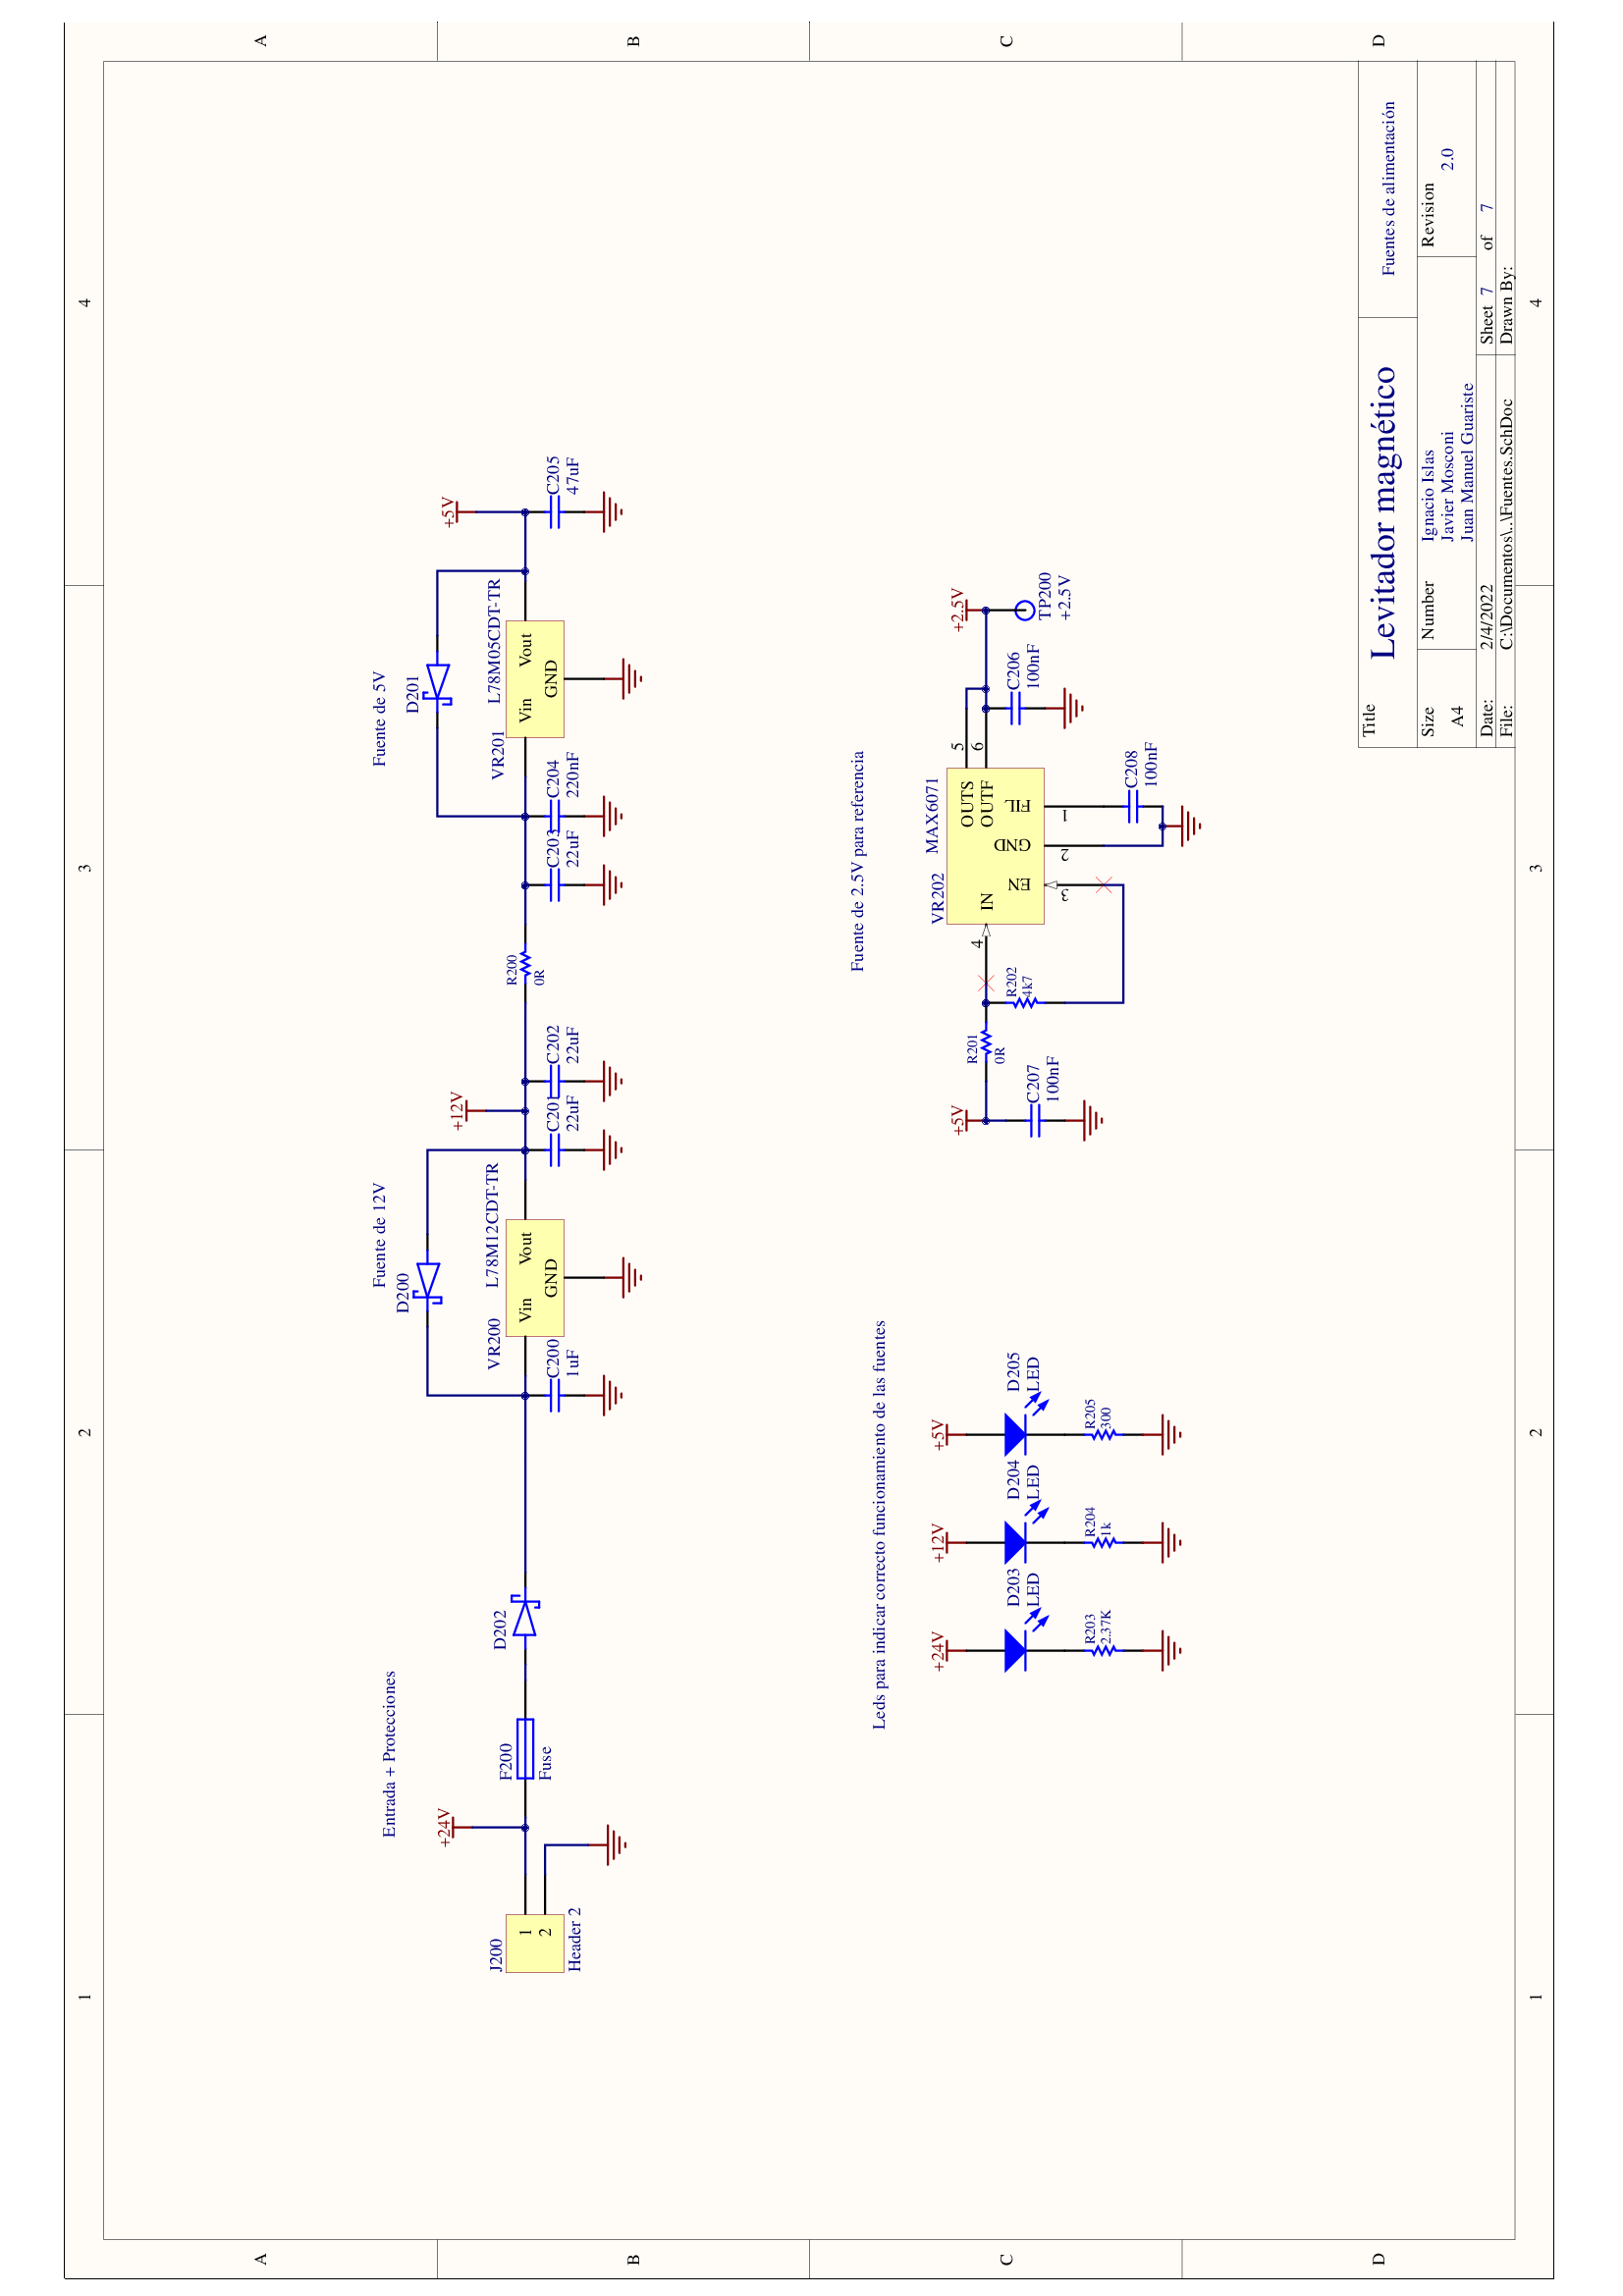
\includegraphics[scale=0.3]{FuentesAliment.png}
	%\caption{Diagrama en bloques de la implementación digital.}
	\label{fig:FuentesAliment}
\end{figure}

\section{ECAD}
\subsection{Modelo 2D}
\subsubsection{Vista Superior}
\begin{figure}[H]
	\centering
	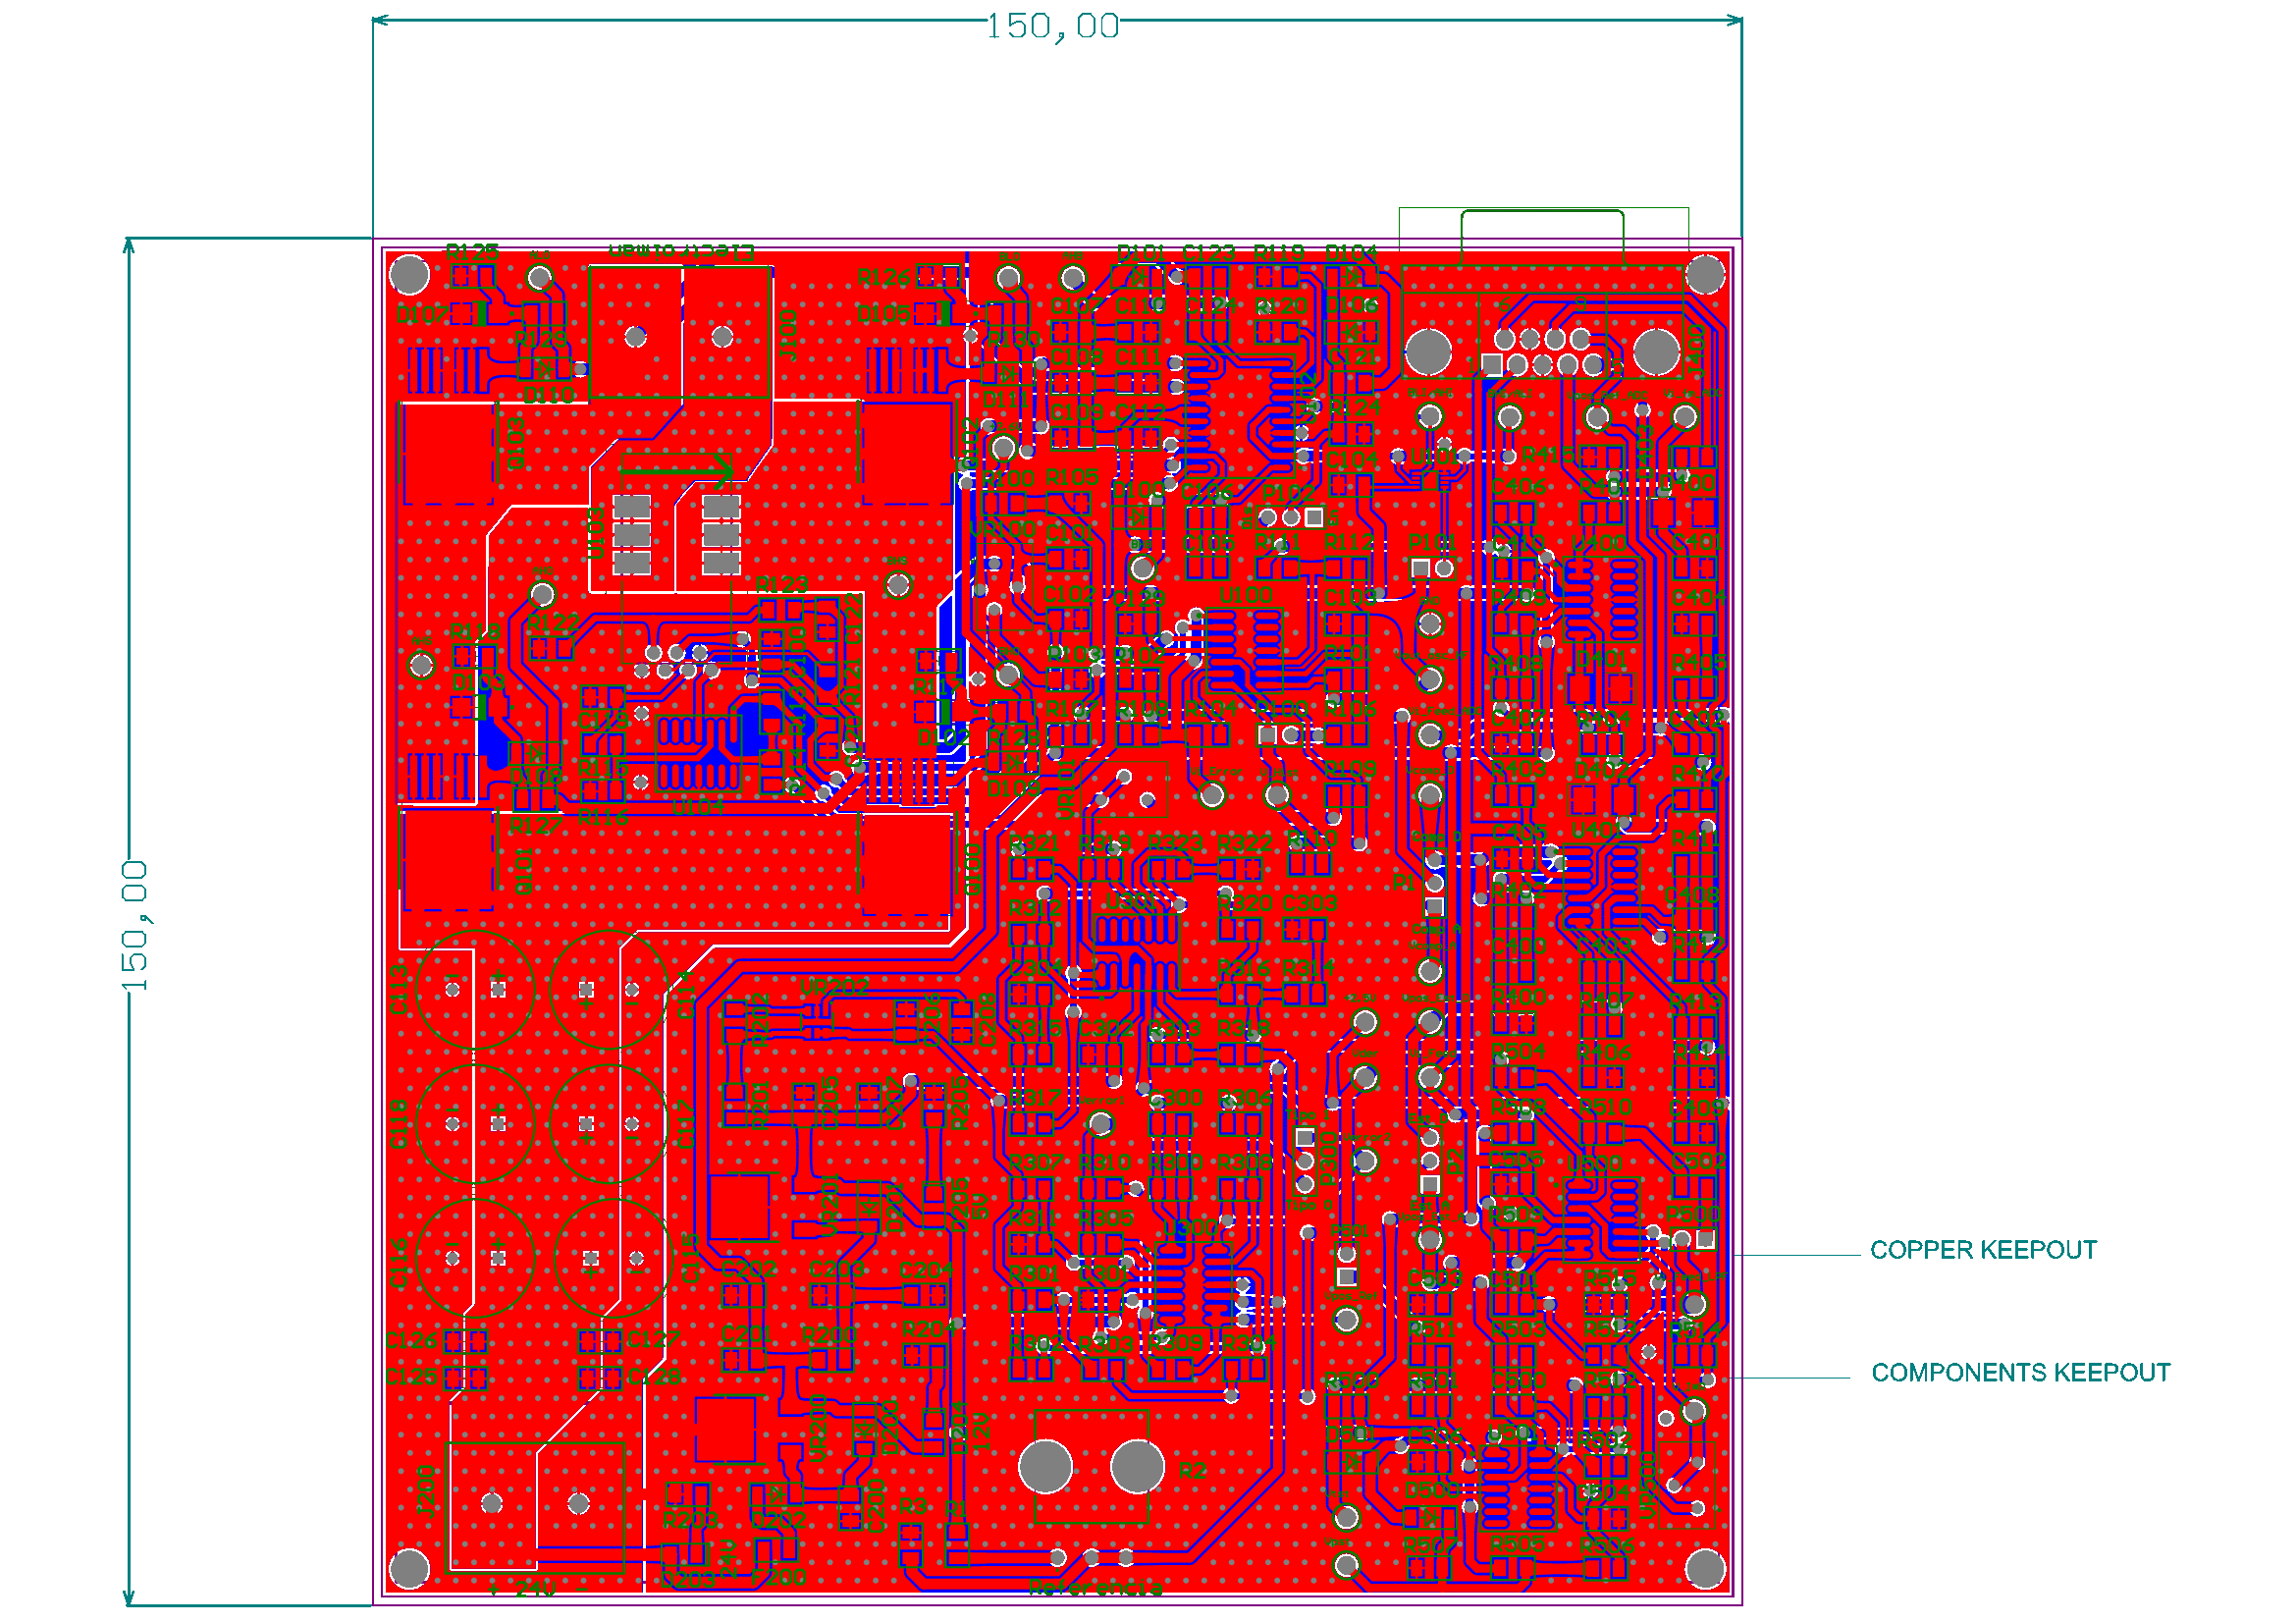
\includegraphics[scale=0.2]{VistSup.png}
	%\caption{Diagrama en bloques de la implementación digital.}
	\label{fig:VistSup}
\end{figure}

\subsubsection{Vista Inferior}
\begin{figure}[H]
	\centering
	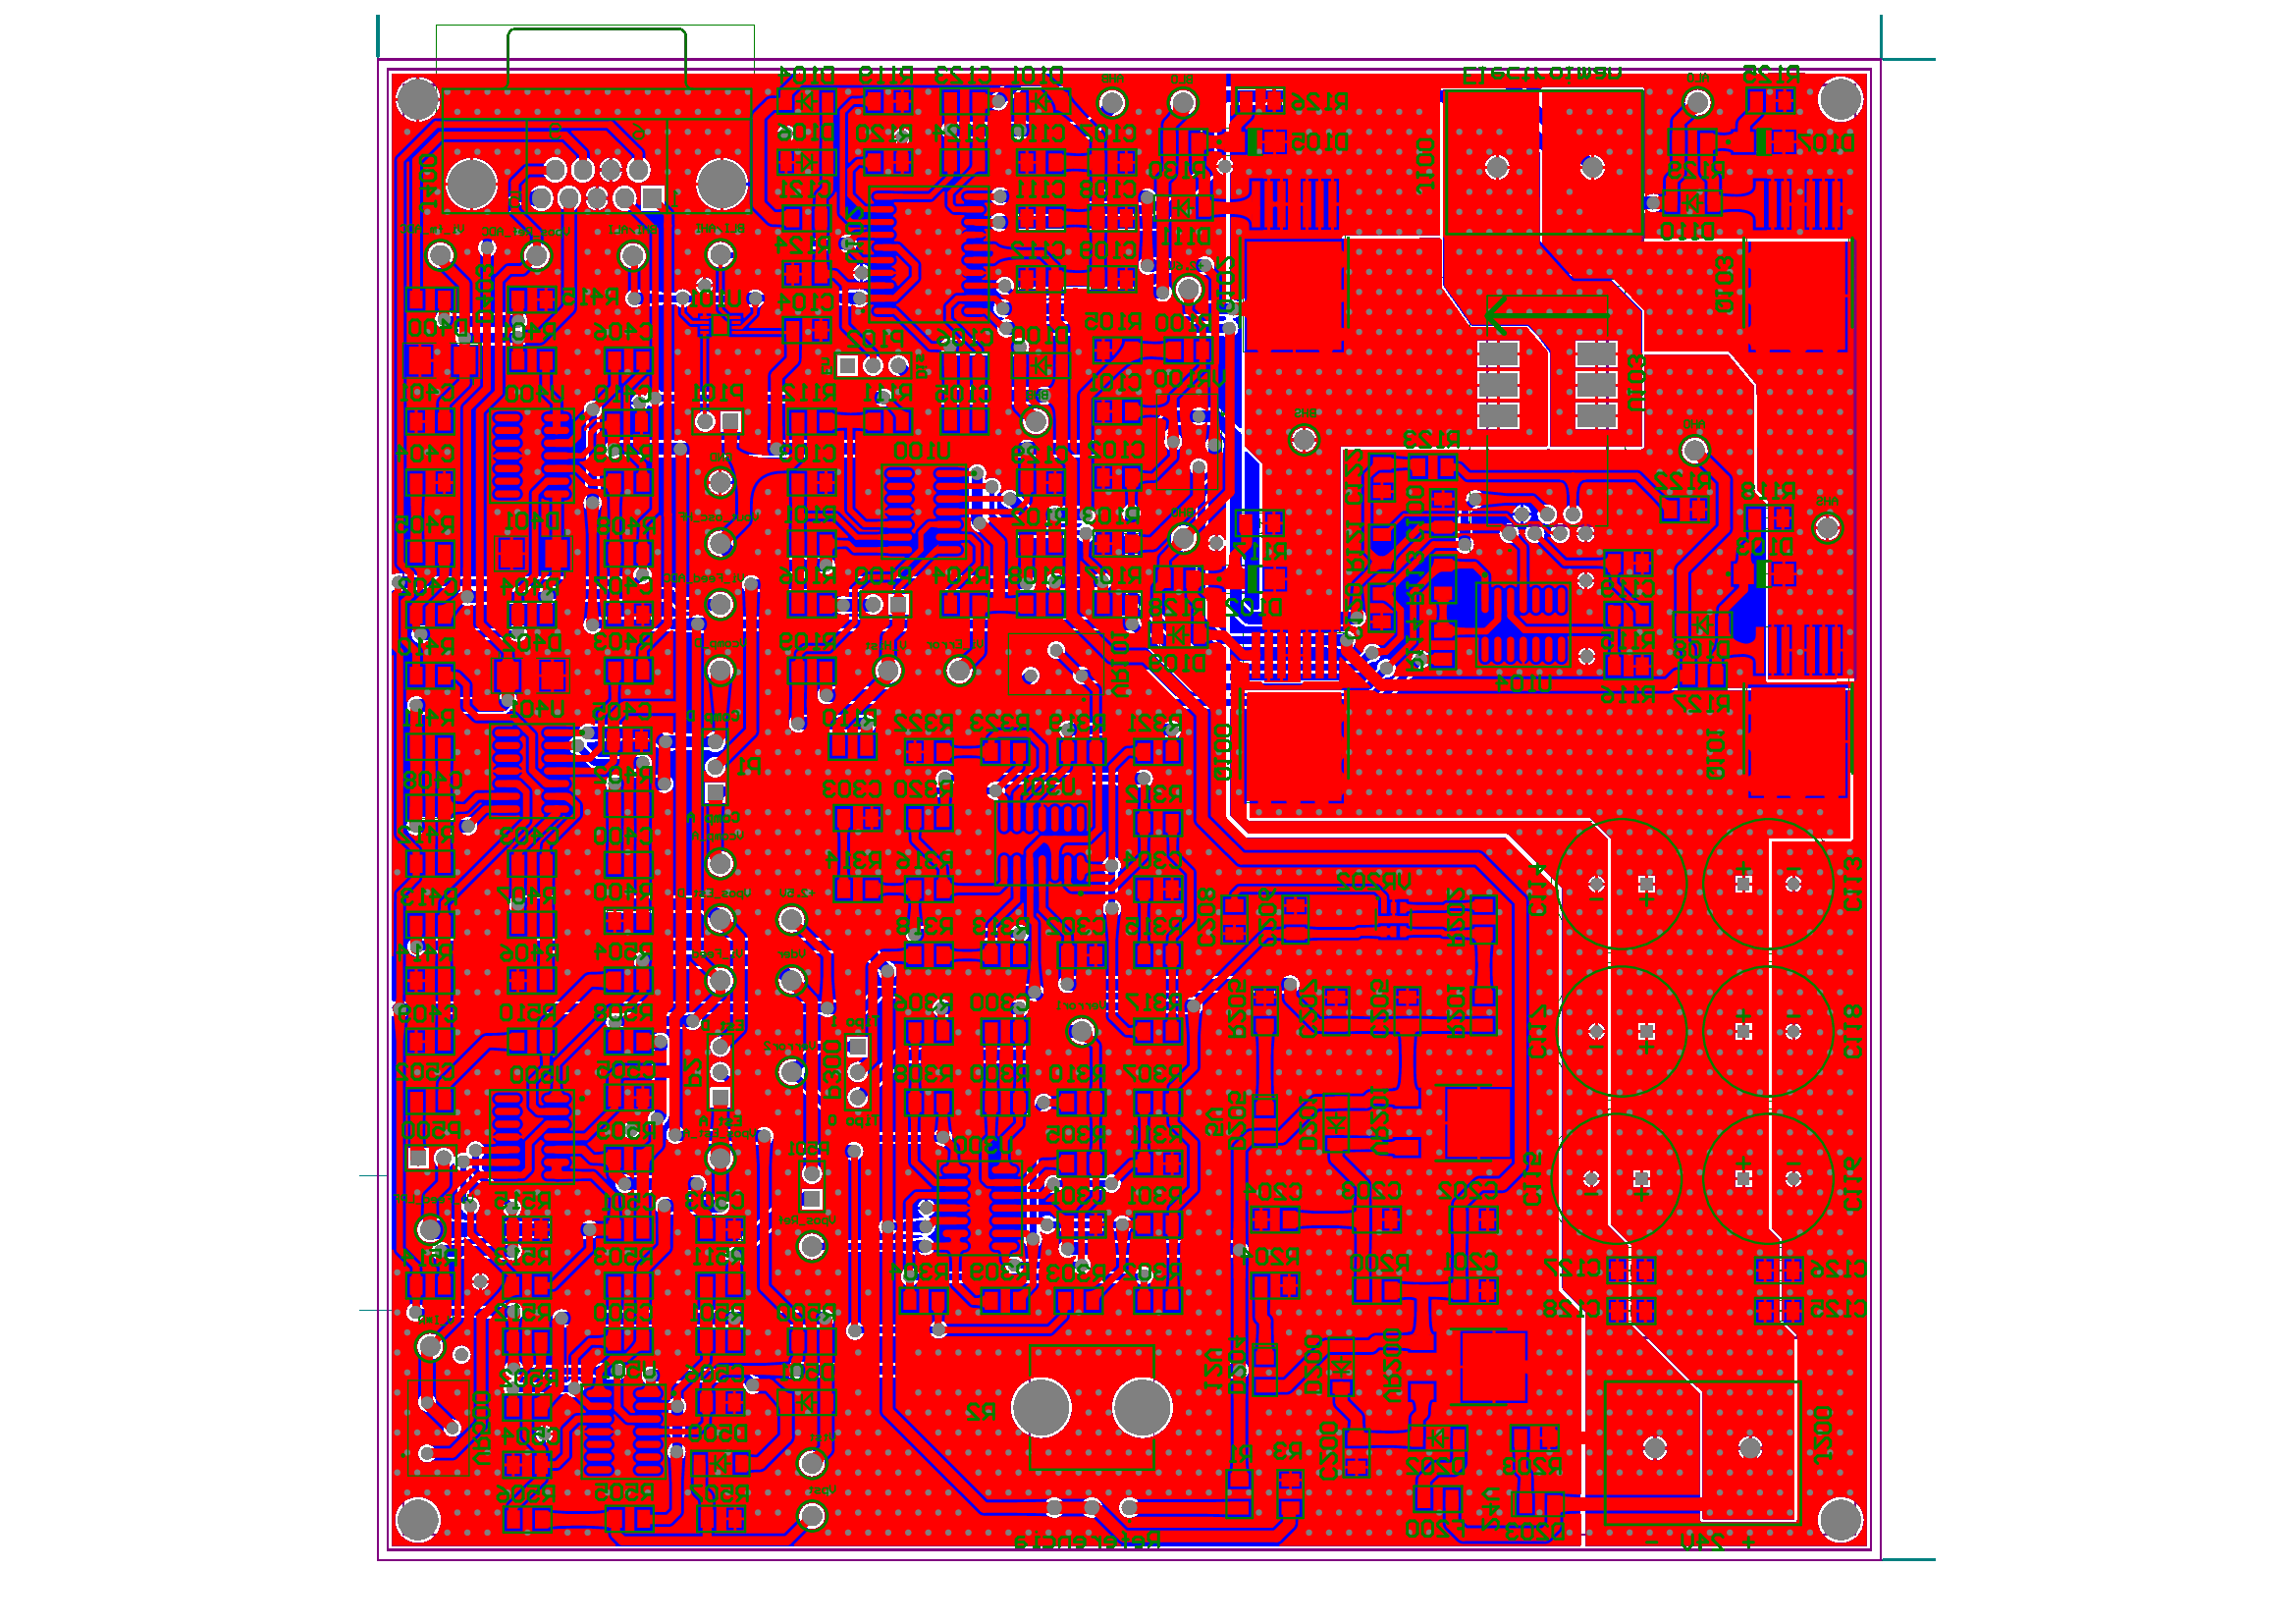
\includegraphics[scale=0.2]{VistInf.png}
	%\caption{Diagrama en bloques de la implementación digital.}
	\label{fig:VistInf}
\end{figure}

\subsection{Modelo 3D}
\subsubsection{Vista Superior}
\begin{figure}[H]
	\centering
	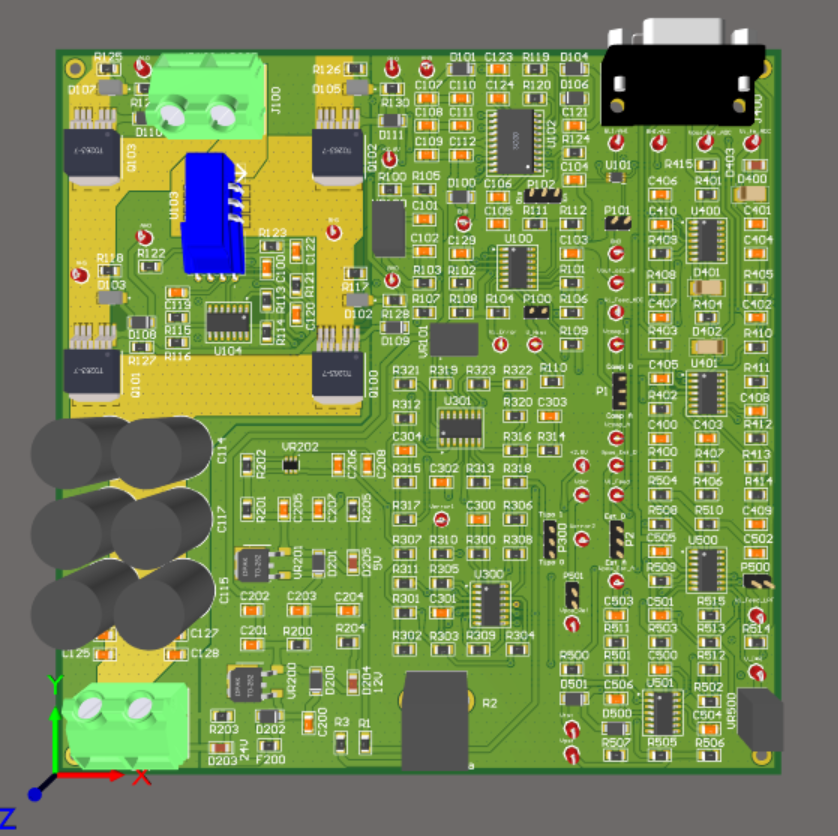
\includegraphics[scale=0.3]{VistSup3D.png}
	%\caption{Diagrama en bloques de la implementación digital.}
	\label{fig:VistSup3D}
\end{figure}

\subsubsection{Vista Inferior}
\begin{figure}[H]
	\centering
	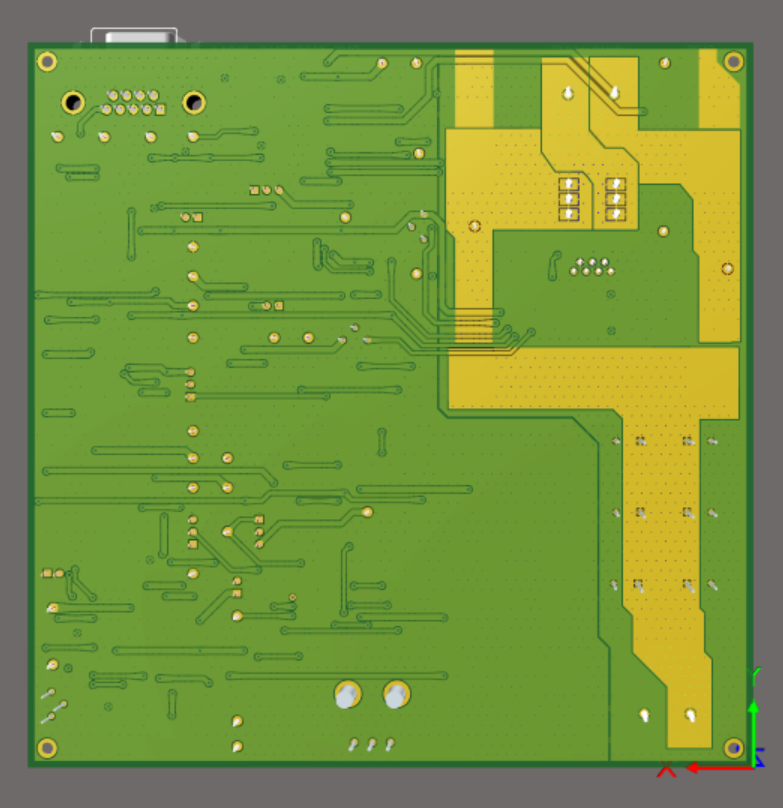
\includegraphics[scale=0.3]{VistInf3D.png}
	%\caption{Diagrama en bloques de la implementación digital.}
	\label{fig:VistInf3D}
\end{figure}

